%% PLEASE INCLUDE ALL IMAGES FROM THE FOLDER  BEFORE COMPILATION %%


\documentclass[a4paper]{article}
\usepackage[a4paper]{geometry}
\usepackage{background}
\usepackage{eso-pic}
\usepackage{enumerate}
\usepackage{amsmath}
\usepackage{amssymb}
\usepackage{underscore}
\usepackage[english]{babel}
\usepackage[utf8]{inputenc}
\usepackage[
backend=biber,
style=alphabetic,
sorting=ynt
]{biblatex}
\addbibresource{201601016.bib}
\title{\huge{\textcolor{red}{\textbf{{THE LIFE OF A BULB : MODEL\hspace{5 mm}\textcopyright}}}}}
\date{\vspace{-5ex}}
\backgroundsetup{
  scale=1,      
  angle=0,       
  opacity=.2,    
  contents={\begin{tikzpicture}[remember picture,overlay]
 \node at ([yshift=11pt,xshift=5pt]current page.center){
\includegraphics[width=5cm]{images.png}};   
    \end{tikzpicture}}
}

\begin{document}

\begin{center}
\Huge{{\bf\textcolor{red}
{PROJECT : CALCULUS}
\vspace{2 cm}
}

\huge{\textbf{
Instructor : {$Prof.$ $Manish$ $K.$ $Gupta$}\\
Course : \textit{SC 107}\\
Calculus With Complex Variable\\
DA-IICT\\
GANDHINAGAR\\
\vspace{4 cm}
AUTHOR : \textit{$SRIKUMAR$ $SASTRY$}\\
ID : \textit{201601016}\\
}
}
}
\vspace*{\fill}
\large{Watermark Courtesy of www.clipartpanda.com}
\end{center}

\begin{figure}
\begin{center}

\includegraphics[width=\linewidth]{light-bulb-quote.jpg}
\end{center}
\caption{\huge{courtesy of the \textit{getwalls.io}}}
\label{fig:bulb1}
\end{figure}
\newpage
\author{
         Srikumar Sastry\\
         201601016,\\
         DAIICT,\\
         GANDHINAGAR\\
      } 
\maketitle
\vspace{2 cm}
\begin{center}
\Huge{\textcolor{blue}{\textbf{IDEA}}}
\begin{quote}
\huge{\textbf{In this Thesis : I will Explain the life of a light bulb.\\
\begin{itemize}
\item Derive the average lifetime of a light bulb.\\
\item Derive the number of bulbs (in a pack) fusing on a given day.\\
\item Estimate the cost of replacing the fused bulbs.
\end{itemize}
}
}
\end{quote}
\end{center}
\vspace*{\fill}
\large{\textbf{Copyright \textcopyright \hspace{2 mm}2016 by Srikumar Sastry
The Problem, Ideas and Equation used in this model 
are solely derived by me. No part of it is taken from internet.
}
}
\newpage
\section{\huge{\textcolor{red}{STATING THE MODEL[1]}}}
\Large{The \textcolor{blue}{Main Model} is as follows :}
\begin{quote}
\Large{Consider a \textit{large} house having 100(\textit{LET}) light bulbs installed inside it.All the light bulbs are installed on the same day and are used simultaneously.\\
1) Find the number of bulbs fusing on a given day.\\
2) Find the cost to replace all fused bulbs on a given day.
\vspace{2 cm}
}
\end{quote}
\subsection{\huge{\textcolor{red}{[1]ASSUMPTIONS}}}
\begin{itemize}
\item \Large{There are 100 light bulbs in total}
\item \Large{All the light bulbs are identical}
\item \Large{All of them are installed at the same time}
\item \Large{All of them are used simultaneously}
\end{itemize}
\vspace*{\fill}
\large{\textbf{NOTE : This model can be generalized for 'N' number of light bulbs}
}
\newpage
\section{\huge{\textcolor{red}{INTRODUCTION}}}
\Large{The Analysis of the \textcolor{blue}{The Light Bulb Model}} Involves the following two principles' : 
\begin{quote}
\begin{center}
\vspace{2cm}
\Large{\textbf{\underline{Principia of PHYSICS}\hspace{1.6 cm}\underline{Principia of MATHS}}}\\
\vspace{2cm}
\begin{tabular}{l||r}
\textbf{Qualitative Analysis} &\textbf{Quantitative Analysis}  \\\\
\textbf{Reasons}&\textbf{Equations}
\end{tabular}
\end{center}
\end{quote}
\vspace{2 cm}
\subsection{\textcolor{red}{\huge{THE PHYSICS LOGIC}}}
\Large{The discipline of \textit{Physics} provide us the exact view of ``What is happening in the model".}
\vspace{1.5 cm}
\Large{It helps us to answer the following questions : }

\begin{tabular}{|l|}
\hline
Why does a Bulb fuse?\\
\hline
Why does the filament break?\\
\hline
How are the different parameters related to each other?\\
\hline
\end{tabular}
\vspace{2 cm}
\begin{enumerate}[(a)]
\item The main reason why a bulb fuses is that the filament inside the bulb breaks.As the filament breaks, the circuit breaks and no current flows thereafter.The filament is made of \textcolor{blue}{Tungsten} which has a high melting point.
\item The main reason why filament breaks is :\\
When the bulb is in \textit{on} mode, immense amount of heat is generated in the filament.This heat \textit{vapourises} the filament by small amount. So, each time the bulb is used, filament vapourises by small amounts. After \textit{considerable} usage, filament becomes very thin and breaks.
\item The process of vapourization is also known as \textcolor{blue}{\textbf{Sublimation}}.
Different metals have different sublimation temperatures.\\
\textit{It has been observed that the rate of sublimation decreases with time at the same temperature and pressure.}\\
Moreover \textit{experimentally} :
\Huge{\textcolor{blue}{$$\frac{dM}{dt}\propto M $$}}
\Large{where $M$ is the mass of Tungsten left.}\\
%\vspace{1 cm}\\
\Large{So basically,\textcolor{blue}{\huge{ $\frac{dM}{dt}$}} represents the rate of sublimation.}\\ 
\vspace{1 cm}\\
So :
\textcolor{blue}{\huge{$$\frac{dM}{dt}=\lambda M$$}}
where $\lambda$ is \textit{sublimation constant} for Tungstun. 
\end{enumerate}
\newpage
\huge{The Graph of the sublimation rate is given by : }
\begin{figure}[h!]
\begin{center}
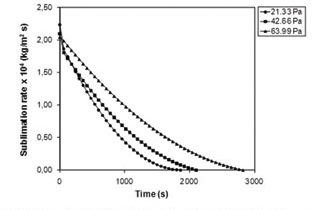
\includegraphics[width=\linewidth]{rate.jpg}
\end{center}
\caption{\huge{courtesy of the \textit{www.scielo.br}}}
\label{fig:bulb2}
\end{figure}
\\The Average pressure inside a bulb is 70kPa.\\
We will consider it as constant for calculation.
\newpage
\subsection{\textcolor{red}{\huge{THE MATHS EXPLANATION}}}
\Large{Physics gave us the equation :}
\begin{center}
\textcolor{blue}{\huge{$\frac{dM}{dt}=\lambda M$}}
\end{center}
Integrating it over finite time period t :
\begin{equation*}
\begin{aligned}
\textcolor{blue}{\huge{\int^{M(t)}_{M
_o} \frac{dM}{M}}} &=\textcolor{blue}{\huge{ \int^t_0 \lambda dt}}\\
\textcolor{blue}{\huge{\log_e{\frac{M(t)}{M_o}}}} &=\textcolor{blue}{\huge{- \lambda t}}\\
\textcolor{blue}{\huge{M(t)}}&=\textcolor{blue}{\huge{M_o e^{-\lambda t}}}
\end{aligned}
\end{equation*}
\Large{Now dM mass that is vapourised in time t is given by :}
\textcolor{blue}{\huge{$$dM = - M_o \lambda e^{-\lambda t} dt$$}}
$\therefore$ The lifetime of the dM mass is :
\textcolor{blue}{\huge{$$dM*t$$}}
%From the equation of $M(t)$ we can see that\\
%$M(t)$ becomes zero at t=$\infty$.\\
%So integral will have limits
$\therefore$ The average life of the Bulb (filament) is:
\begin{equation*}
\begin{aligned}
\tau &= \frac{Sum \mbox{ } of \mbox{ } lives \mbox{ } of \mbox{ } all \mbox{ } dM \mbox{ } masses}{Total \mbox{ } mass \mbox{ } of \mbox{ } filament}\\
\textcolor{blue}{\tau}&=\textcolor{blue}{\frac{\int dM*t}{M_o}}\\
\textcolor{blue}{\tau}&=\textcolor{blue}{\frac{\int^\infty_0 -M_o\lambda e^{-\lambda t} t dt}{M_o}}\\
\textcolor{blue}{\tau}&=\textcolor{blue}{\int^\infty_0 -\lambda e^{-\lambda t} t dt}\\
&\mbox{Integrating by Parts : }\\
\textcolor{blue}{\tau}&=\textcolor{blue}{-\lambda (t \int e^{-\lambda t} dt - \int \int e^{-\lambda t}dt dt)}\\
\end{aligned}
\end{equation*}
\newpage
After putting the limits : 
\textcolor{blue}{$$\tau=\frac{1}{\lambda}\mbox{ (Average life time)}$$}
\vspace{2 cm}\\
\textcolor{green}{\huge{Calculating the probability of bulb fusing on a day}}
\vspace{1 cm}\\
Now there are 100 identical bulbs in the house.\\
Each of them will have $\tau$ as its average lifetime.\\
\textbf{THE AVERAGE LIFE OF A TYPICAL LIGHT BULB IS AROUND 125 DAYS}
(used at 8 hours a day)\\
\huge{That is $\tau=\frac{1}{\lambda}=1000\mbox{\textbf{(hours)}}$}\\
\vspace{1 cm}\\
\textbf{Using Poisson distribution \cite{Moi60} : }\\
\huge{Probability of one bulb fusing on $k^{th}$ day $=$
\textcolor{blue}{$$\frac{e^{-\tau} \tau^k}{k!}$$} \\
Probability that n(of 100) bulbs fuse on $k^{th}$ day $=$
    \textcolor{blue}{$$\binom{100}{n}(\frac{e^{-\tau} \tau^k}{k!})^n$$}
\begin{figure}[h!]
\begin{center}
THE POISSON DISTRIBUTION
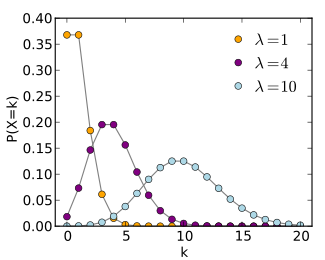
\includegraphics[width=\linewidth]{Poisson.png}
\end{center}
\caption{\huge{courtesy of the \textit{en.wikipedia.org}}}
\label{fig:bulb3}
\end{figure}
\newpage
$\therefore$ Number of Bulbs fusing on $k^{th}$ day $=$
Value of n that we get from - \\
\textcolor{blue}{$$P_n=\left \lfloor{max(\binom{B}{n}(\frac{e^{-\tau} \tau^k}{k!})^n)}\right \rfloor$$}
Where B is the number of bulbs left after k-1 days.\\
\vspace{1 cm}\\
n can be calculated by -
\textcolor{blue}{\textbf{$$\frac{P_n}{P_{n+1}}>1$$}}
\textcolor{blue}{\textbf{$$\frac{P_n}{P_{n-1}}>1$$}}
$\therefore$ The cost of replacing bulbs on $k^{th}$ day is =\\
\textcolor{blue}{\textbf{\huge{$$C_k=n * \mbox{ cost of one bulb}$$}}}
\vspace*{\fill}\\
\large{\textbf{NOTE : No part of this calculation can be found on Internet.}
}
\newpage
\section{\huge{\textcolor{red}{APPLICATIONS}}}
\LARGE{This Solution can be expanded to daily life electric devices which need frequent maintenance.\\
The approach has been defined.We only need to know the dependence of parameters on one another.Then we can easily derive for other devices.\\ It can be used to keep a check on money that is spent on the electric devices on daily basis.\\
This solution can also be used to further study the functioning of different electric devices (not only bulbs).}
\section{\huge{\textcolor{red}{CONCLUSION}}}
\LARGE{Though this model involves a number of assumptions,\\
it uses powerful technique of integration and knowledge of probability.\\
At last we arrive at a satisfied solution,\\
which can be used in daily lives.
}
\newpage
\printbibliography
\end{document}